\documentclass[man]{apa2}

\usepackage{url}
\usepackage{apacite}
\usepackage{pslatex}
\usepackage{pdfsync}
\usepackage{apacite}
\usepackage{amsmath}
\usepackage{graphicx}
\usepackage{topcapt}
\usepackage{color}


%\usepackage{setspace}
%\usepackage[margin=1in]{geometry}
%
%\doublespacing

\title{Negation is only hard to process when it is pragmatically uninformative}
\author{Ann E. Nordmeyer, Noah D. Goodman, and Michael C. Frank}
\affiliation{Department of Psychology, Stanford University}

\shorttitle{Pragmatics of negation}

\abstract{Negation is a fundamental element of language and logical systems, but processing negative sentences can be challenging. Previous work suggests that a supportive context can mitigate the processing costs of negation.  We investigate the role of context on negative sentences by measuring the processing cost of negation in different contexts.  We find that a supportive visual context has a graded effect on negation processing.  Reaction times to respond to both positive and negative sentences were predicted by participants' descriptions of the same stimuli.  Our data suggest that in the right context, representing negation may be less difficult than previously supposed. }  
%A model of the informativeness of an utterance in context predicted participants' descriptions of the stimuli as well as reaction times to evaluate sentences.  




\acknowledgements{This material is based upon work supported by the National Science Foundation Graduate Research Fellowship. }



\begin{document}
\maketitle

%%%%%%%%% INTRO %%%%%%%%% 
\section{Introduction}

Language is a powerful tool that allows us to describe not only the state of the world as we see it, but also the world as it is not.  It would be strange for a barista to say ``We don't have any chai today'' unless I'm a regular who always orders chai.  Negative sentences tend to be uninformative, except when expectations are violated.

%Could cut this down -- remove EEG stuff or condense?
Although negation is critical for communicating many meanings and is an important component of logical systems, processing negative sentences can be slow and effortful.  Classic works shows that participants who are asked to evaluate the truth of a sentence describing a picture take significantly longer to evaluate negative sentences compared to positive ones \cite{hclark1972, carpenter1975, just1971, just1976}. In EEG experiments, sentences in which the final noun is semantically unexpected elicit an N400 response; this response is found even when a negative makes the sentence logically true (e.g.\ ``A robin [is/is not] a truck'')---suggesting that negation is slow to integrate with the rest of the sentence \cite{fischler1983, ludtke2008}.  Similar results have been found in probe-recognition tasks \cite{kaup2003, kaup2006, hasson2006}. This work could been taken as evidence that representing logical relations is cognitively difficult.

There is a critical difference, however, between sentences presented on a computer in the lab and speech that we hear in the real world. According to Grice's Cooperative Principle \cite{grice1975}, listeners expect speakers to produce utterances that are truthful, relevant, and informative.  Negative sentences presented without context violate this principle.  If the barista in our earlier example says ``we don't have chai today'' to a customer who always orders coffee, this utterance would be neither relevant nor informative.  In general, listeners should expect speakers to produce negation when expectations are violated.

Congruent with this Gricean account, a number of studies have shown that a supportive context mitigates the processing cost of negation \cite{wason1965, glenberg1999, ludtke2006, nieuwland2008, dale2011}. Some contexts are more effective than others at reducing processing demands. For example, contexts that explicitly mention a negated characteristic \cite{ludtke2006} or that present the negation within a dialogue \cite{dale2011} elicit faster reaction times.  But although these findings are congruent with the idea that pragmatic expectations are the source of negation's processing cost, they do not directly test that hypothesis.  The goal of our current work is to make such a test.

%Maybe move some of this to the GD
%What is the mechanism by which context influences the processing of negation?  We propose that negative sentences are more informative in contexts that set up a strong expectation that is violated. If the processing cost of negation is pragmatic, then more informative negative sentences should elicit smaller reaction times. How should we quantify informativeness in context? Recent modeling work quantifies pragmatic reasoning in simple experimental contexts \cite{frank2012,goodman2013}. The assumption underlying this work is that speakers are informative---they will produce utterances that will pick out smaller subsets of the context, leaving as little ambiguity as possible for the listener.  We use this definition of informativeness to provide a quantitative interpretation of our hypothesis.

%MOVE THIS:
%To link pragmatic expectations to reaction time, we assume that reaction time is proportional to \emph{surprisal}. Surprisal is an information-theoretic measure of the amount of information carried by an event (in this case, an utterance in some context) based on its probability. Surprisal has been used effectively to predict reaction times from probabilistic models \cite{levy2008}; in this work, we directly measure the probability of an utterance occurring by eliciting descriptions of our stimuli from our participants.

We test the hypothesis that pragmatic surprisal explains the processing cost of negative sentences.  Participants viewed an array of characters who were identical except for the presence or absence of some feature, parametrically varying the base rate of these features across trials.  Participants were asked to either read and evaluate sentences about these characters (listener condition), or to complete sentences about the characters (speaker condition).  If participants in our listener condition have Gricean expectations about the sentences in our experiment, they should be faster to evaluate sentences that are more probable based on the responses of participants in the speaker condition.  Consistent with this prediction, we found that context has a graded effect on the processing of negative sentences, and that participants' descriptions of the sentences predicted the relationship between context and reaction time.  These results suggest that the processing cost associated with logical terms such as negation may be driven by pragmatic rather than representational difficulties.
%A model of pragmatic informativeness supports our hypothesis that this relationship is driven by the relative informativeness of a sentence in context.  
%These results provide novel, quantitative support for a pragmatic account of the processing of negative sentences.


%
%\section{Experiment 1: Context vs. No Context}
%
%To test whether non-linguistic contextual expectations alleviate the processing cost of negative sentences, we constructed a simple sentence verification task based on \citeA{hclark1972}.  Previous studies of the relationship between context and negation have required participants to actively engage with the context, either by describing pictures \cite{wason1965} or reading sentences \cite{glenberg1999}.  Here, participants passively viewed a visual context, providing further evidence that the effects of context on negative sentence processing are robust in a wide variety of contexts.
%
%\subsection{Method}
%
%\subsubsection{Participants}
%
%We recruited 100 participants to participate in an online experiment through the Amazon's Mechanical Turk (mTurk) website.\footnote{Previous work has shown that mTurk is an effective tool for collecting RT data \cite{crump2013}.}  Participants ranged in age from 18-65; 63 were male and 37 female.  We restricted participation to individuals in the United States. We paid participants 30 cents to participate, which took approximately 5 minutes to complete.  
%
%\subsubsection{Stimuli}
%
%\begin{figure}[t]
%\begin{center} 
%\includegraphics[width=3.25in]{figures/negatron_trialfig2.pdf}
%\caption{\label{fig:trial} An example trial, consisting of two separate slides (shown sequentially): a context slide and a trial slide for a true negative trial. }
%\vspace{-5mm}
%\end{center} 
%\end{figure}
%
%Twenty-eight trial items were created in which a character was shown holding either two of the same common, recognizable objects (e.g.\ two apples), or holding nothing.  On each trial a sentence of the form ``[NAME] [has/has no] [ITEM]'' was written.  Half of the sentences were positive and half were negative, and they were paired with pictures such that half were true and half were false.  The experiment was fully crossed, with participants receiving seven true positive, seven false positive, seven true negative and seven false negative sentences in a randomized order over the course of the study.  
%
%Participants were randomly assigned to the ``no context'' condition or the ``context'' condition.  Participants in the no context condition saw a blank screen with a fixation cross before each trial, while participants in the context condition viewed a context slide.  The context slide showed three characters, each holding the same two identical items.  The characters all differed from the trial character and from each other in hair and shirt color.  A sentence instructed participants to ``Look at these [boys/girls]!'' (Fig.\ \ref{fig:trial}).  
%
%
%\subsubsection{Procedure}
%Participants were first presented with an instructions screen which described the task and informed them that they could stop at any time.  Once they accepted the task, they were given eight positive sentence practice trials with feedback about incorrect responses. 
%
%In each trial, participants saw a context (3s) and then a picture and a sentence. They were asked to read the sentence and respond as quickly and accurately as possible with a judgment of whether it was true or false when applied to the picture.  We recorded reaction times for each trial, measured as the time from when the picture and sentence were presented to the moment when the response was made.
%
%\subsubsection{Data Processing}
%We excluded from analysis 6 participants who did not list English as their native language, 7 participants for having participated in a previous pilot study, and 4 participants for having an overall accuracy of below 80\%.  Thus, data from a total of 83 participants were analyzed.  We also excluded trials with RTs greater than 3 standard deviations from the log-transformed mean.  
%
%\subsection{Results \& Discussion}
%
%\begin{figure}
%\begin{center} 
%\includegraphics[width=3.25in]{figures/study1_linegraph.pdf}
%\caption{\label{fig:e1line} Reaction times for each trial type across different conditions.  Responses to true sentences are shown on the left, and false sentences are shown on the right.  Negative sentences are shown in grey, and positive sentences in black.  Error bars show 95\% confidence intervals.}
%\end{center} 
%\end{figure}
%
%Negative sentences were difficult to process when presented without context; in context, this effect disappeared (Fig.\ \ref{fig:e1line}).  This result is congruent with previous work on sentence verification, which has also found a main effect of negation \cite<e.g.>{hclark1972} and with work examining the role of context in negation \cite<e.g.>{wason1965, nieuwland2008, dale2011}.  
%
%To examine the reliability of these findings, we fit a linear mixed-effects model to participants' reaction times.  We examined the interaction between sentence type, truth value, and context on reaction times.\footnote{All mixed-effects models were fit using the lme4 package in R version 2.15.3.  The model specification was as follows: \texttt{RT $\sim$ sentence~$\times$~truth~$\times$~context + (sentence~$\times$~truth~\textbar~subject) +  (sentence~$\times$~truth~\textbar~item)}.  Significance was calculated using the standard normal approximation to the $t$ distribution \cite{barr2013}. Data and analysis code can be found at FILL THIS IN LATER} Results of this model show a main effect of truth value, with significant faster reaction times for true sentences compared to false sentences ($\beta= -196$, $p< .001$).\footnote{Coefficient weights are interpretable in milliseconds.}  Although there was no main effect of negation across both conditions, there was an interaction between sentence type and truth value ($\beta= 260$, $p< .001$), replicating the finding that participants respond fastest to true positive sentences but slowest to true negative sentences \cite{hclark1972}.  Critically, there was a significant 3-way interaction between context condition, sentence type, and truth value ($\beta= -227$, $p< .01$), suggesting that this interaction was primarily driven by the slow RTs for true negative sentences in the no context condition.  
%
%To understand why context had the strongest effect on true negative sentences, consider what a true negative trial looks like in the no context condition.  These are trials in which the participant has no expectation about what the character might be holding, because no context was provided to set up such an expectation.  The participant would then see a picture of an empty-handed boy with the sentence ``Bob has no apples.''  These types of trials likely cause participants to falter because there is no reason for ``apples'' to be mentioned at all.  However, when a participant first views a context such as the one in Fig.\ \ref{fig:trial}, they can form an expectation that boys typically have apples.  Now, when participants see a boy with no apples, a sentence such as ``Bob has no apples'' makes sense.
%
%Experiment 1 contributes to a body of evidence suggesting that negative sentences are more felicitous when they negate an expectation, and that such expectations can be set up by an appropriate context.  In Experiment 2, we examine how systematically manipulating the strength of the context might produce changes in reaction times by altering the expectations created by the context.  

%\section{Experiment}


%Are all contexts be equally helpful in processing negation? In Experiment 1, we parametrically manipulated the context of negative sentences to examine how the strength of the expectations set up by the context influences the processing of negation.  
%Previous studies of the relationship between context and negation have required participants to actively engage with the context, either by describing pictures \cite{wason1965} or reading sentences \cite{glenberg1999}.  Here, participants passively viewed a visual context, providing further evidence that the effects of context on negative sentence processing are robust in a wide variety of contexts.
%On each trial, participants saw four characters, identical except for the presence or absence of familiar items (e.g. some characters held apples, while others held nothing).  After several seconds, a red box appeared around one of the characters, and a sentence appeared about that picture.  Participants were instructed to decide as quickly as possible whether the sentence was true or false of the indicated picture.  

%Across trials, we manipulated the proportion of characters who possessed the target items.  If the context gives participants a glimpse into the world that each trial exists in, this represents a small sample of the base rate of what the characters in this world look like.  By manipulating this base rate, we can change peoples' expectations about the trial character.  If the effect of context on negation is due to the relative informativeness of an utterance based on the context, we should expect to see a relationship between the strength of the context and reaction time. 


\section{Method}

\subsection{Participants} 

%NOTE: These ns are correct & checked
We recruited 489 participants (262 male and 224 female, three declined to report gender; ages 18 -- 65+) to participate in an online experiment through the Amazon's Mechanical Turk (mTurk) website.  We restricted participation to individuals in the US and paid 50 cents for this 10 minute study.  Participants were randomly assigned to either the speaker condition (n = 296) or the listener condition (n = 193).

\subsection{Stimuli}

\begin{figure}[t]
\begin{center} 
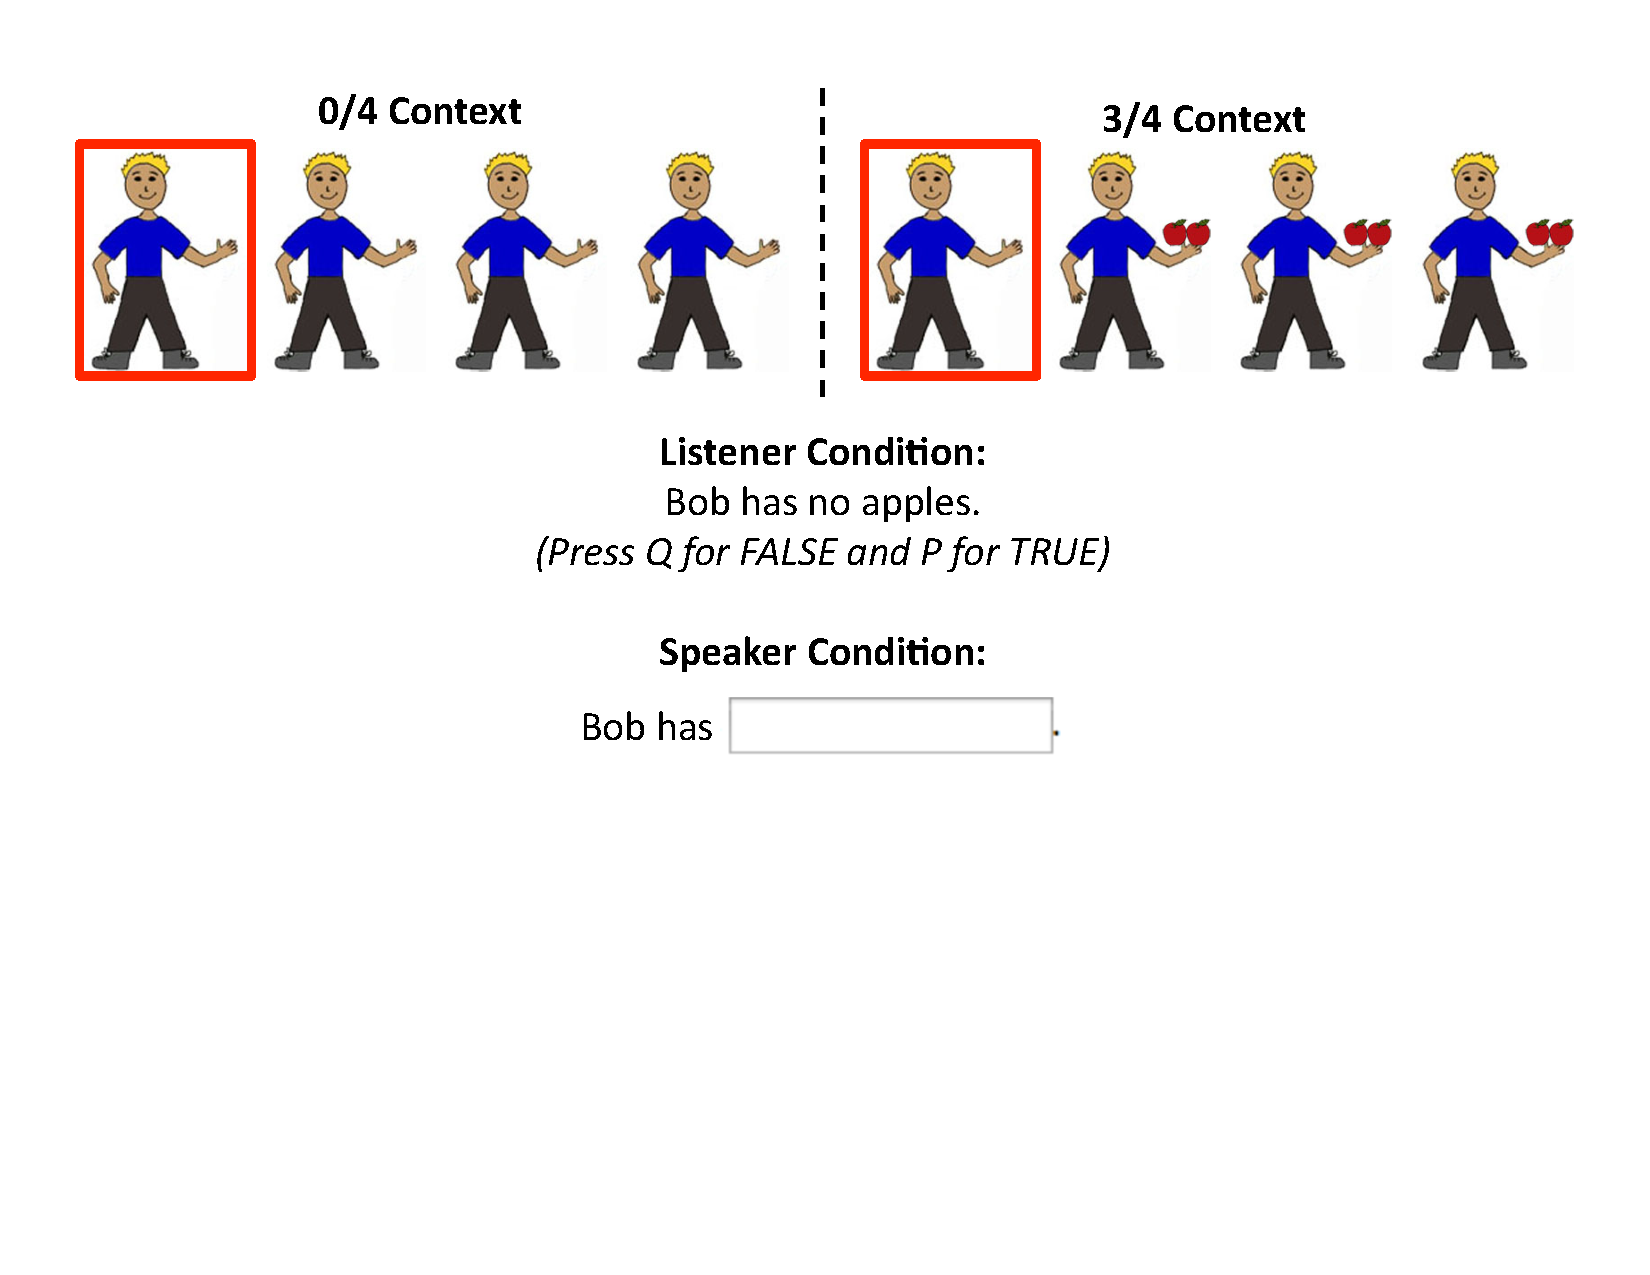
\includegraphics[width=4in]{figures/trialfig.pdf}
\caption{\label{fig:trial} An example of a true negative trial with a 3/4 context. Participants in the listener condition were asked to read and evaluate a sentence like the one above.  Participants in the speaker condition saw the same stimuli but were asked to complete a sentence such as ``Bob has  \textunderscore\textunderscore\textunderscore\textunderscore\textunderscore\textunderscore\textunderscore\textunderscore\textunderscore\textunderscore.''}
\vspace{-5mm}
\end{center} 
\end{figure}

Thirty-two trial items were created in which characters were shown holding either two of the same common, recognizable objects (``target items'', e.g. two apples), or holding nothing.  Within each trial, all characters were identical except for the presence or absence of objects; characters varied in appearance (e.g. skin tone, hair color, clothing, gender) across trials.\footnote{Our previous work indicates that the results reported here are robust to a number of changes to the stimuli, including whether the context characters varied in appearance or not.  Results from these previous experiments can be seen in \citeA{nordmeyer2014}.}

A within-subjects factor determined what type of context participants saw on each trial.  The context condition determined the proportion of characters who were holding target items.  Context conditions showed $\frac{0}{4}$, $\frac{1}{4}$, $\frac{2}{4}$, $\frac{3}{4}$, or $\frac{4}{4}$ of the characters holding objects. The order of characters was shuffled on each trial, with the referent of the sentence appearing in a random position.  

\subsubsection{Listener Condition}
For participants in the listener condition, on each trial a sentence of the form ``[NAME] [has/has no] [ITEM]'' appeared.  Half of the sentences were positive and half were negative, and they were paired with pictures such that half were true and half were false.  The experiment was fully crossed, with participants receiving eight true positive, eight false positive, eight true negative and eight false negative sentences distributed equally across context types in a randomized order over the course of the study.  

\subsubsection{Speaker Condition}
Participants in the speaker condition saw the same images paired with an incomplete sentence (e.g. ``[NAME] has $\rule{3cm}{0.15mm}$.''). In half of the trials, the highlighted picture was holding target items, and in half of the trials, the highlighted picture was holding nothing.  The experiment was fully crossed such that target characters appeared with or without target items an equal number of times in each context type.  

\subsection{Procedure}
Participants were first presented with a brief overview screen which explained that they would play a language game.  Once participants accepted the task, they were randomly assigned to either the listener condition or the speaker condition, and saw a more detailed instructions screen which explained the task and informed them that they could stop at any time.  

\subsubsection{Listener Condition}

In the listener condition, participants first saw eight positive sentence practice trials with feedback about incorrect responses before beginning the test trials. 

In each test trial, participants saw an array of four pictures presented in a randomized order.  Participants were told to look at these pictures for four seconds, at which point a red box appeared around one of the pictures.  One second later, a sentence about that picture appeared.  Participants were told to read the sentence and respond as quickly and accurately as possible with a judgment of whether it was true or false when applied to the highlighted picture.  We recorded reaction times for each trial, measured as the time from when the sentence was presented to the moment when the response was made.\footnote{The listener condition of the experiment can be viewed at 
FIXME (I can't get the link to work, it is clickable but sends to the wrong place due to the line break??) \url{https://langcog.stanford.edu/expts/AEN/negatron_production2/negatron.html}.}

\subsubsection{Speaker Condition}

In each trial, participants saw an array of four pictures: The target pictures and three context pictures presented in a random order.  Participants were told to look at these pictures for four seconds, at which point a red box appeared around one of the pictures.  One second later, an incomplete sentence appeared.  Participants were told to finish the sentence (by typing into a small text box) using only a few words, in a way that would help someone else identify the character in the red box if they saw the pictures in a different order.\footnote{The listener condition of the experiment can be viewed at 
FIXME (I can't get the link to work, it is clickable but sends to the wrong place due to the line break??) \url{https://langcog.stanford.edu/expts/AEN/negatronv20/negatron.html}.}
  

 
 \subsection{Data Processing} 
  
We excluded 18 participants who did not list English as their native language and two participants from the listener condition for having an overall accuracy below 80\%, leaving a total of 469 participants for analysis (186 in listener condition, 283 in speaker condition). 

\subsubsection{Listener Condition}
We excluded trials with RTs greater than 3 standard deviations from the log-transformed mean.  

\subsubsection{Speaker Condition}
Affirmative responses labeling the target feature were coded as ``positive'' (e.g. ``apples'', ``two apples'', ``red apples'', etc.).  Responses with a negative element (``no'', ``not'', ``nothing'', ``empty'', or ``zero'') were coded as ``negative''.  All other responses (e.g. descriptions of the characters' clothing or hair color) were coded as ``other''.  Codes were hand-checked to ensure that label synonyms or spelling errors were coded correctly.  

Due to the Gricean nature of the intuition---which lead us to consider a truthful speaker as well---we focused on predicting the processing of true or correct sentences.   We calculated the proportion of positive sentences describing characters who possessed target items, and the proportion of negative sentences describing characters with nothing, creating a probability distribution for true positive and true negative utterances.  We then used this to calculate the surprisal (an information-theoretic measure of the amount of information carried by an event; see \cite{levy2008}) of a positive or negative sentence for each trial type.  

\begin{equation}\label{eq:surprise}
Surprisal = -\log(P(sentence)).
\end{equation}

%NOTE: We should talk about the best way to present the speaker data.  What I've done here is pretty sparse (I really just jump right to surprisal, describing how we calculate that here and then describing the relationship between surprisal and RT in the results section.  I'm wondering if we should present a table of the probabilities in response to each trial type, though?)

\section{Results}

\subsection{Listener Condition}

\begin{figure}[t]
\begin{center} 
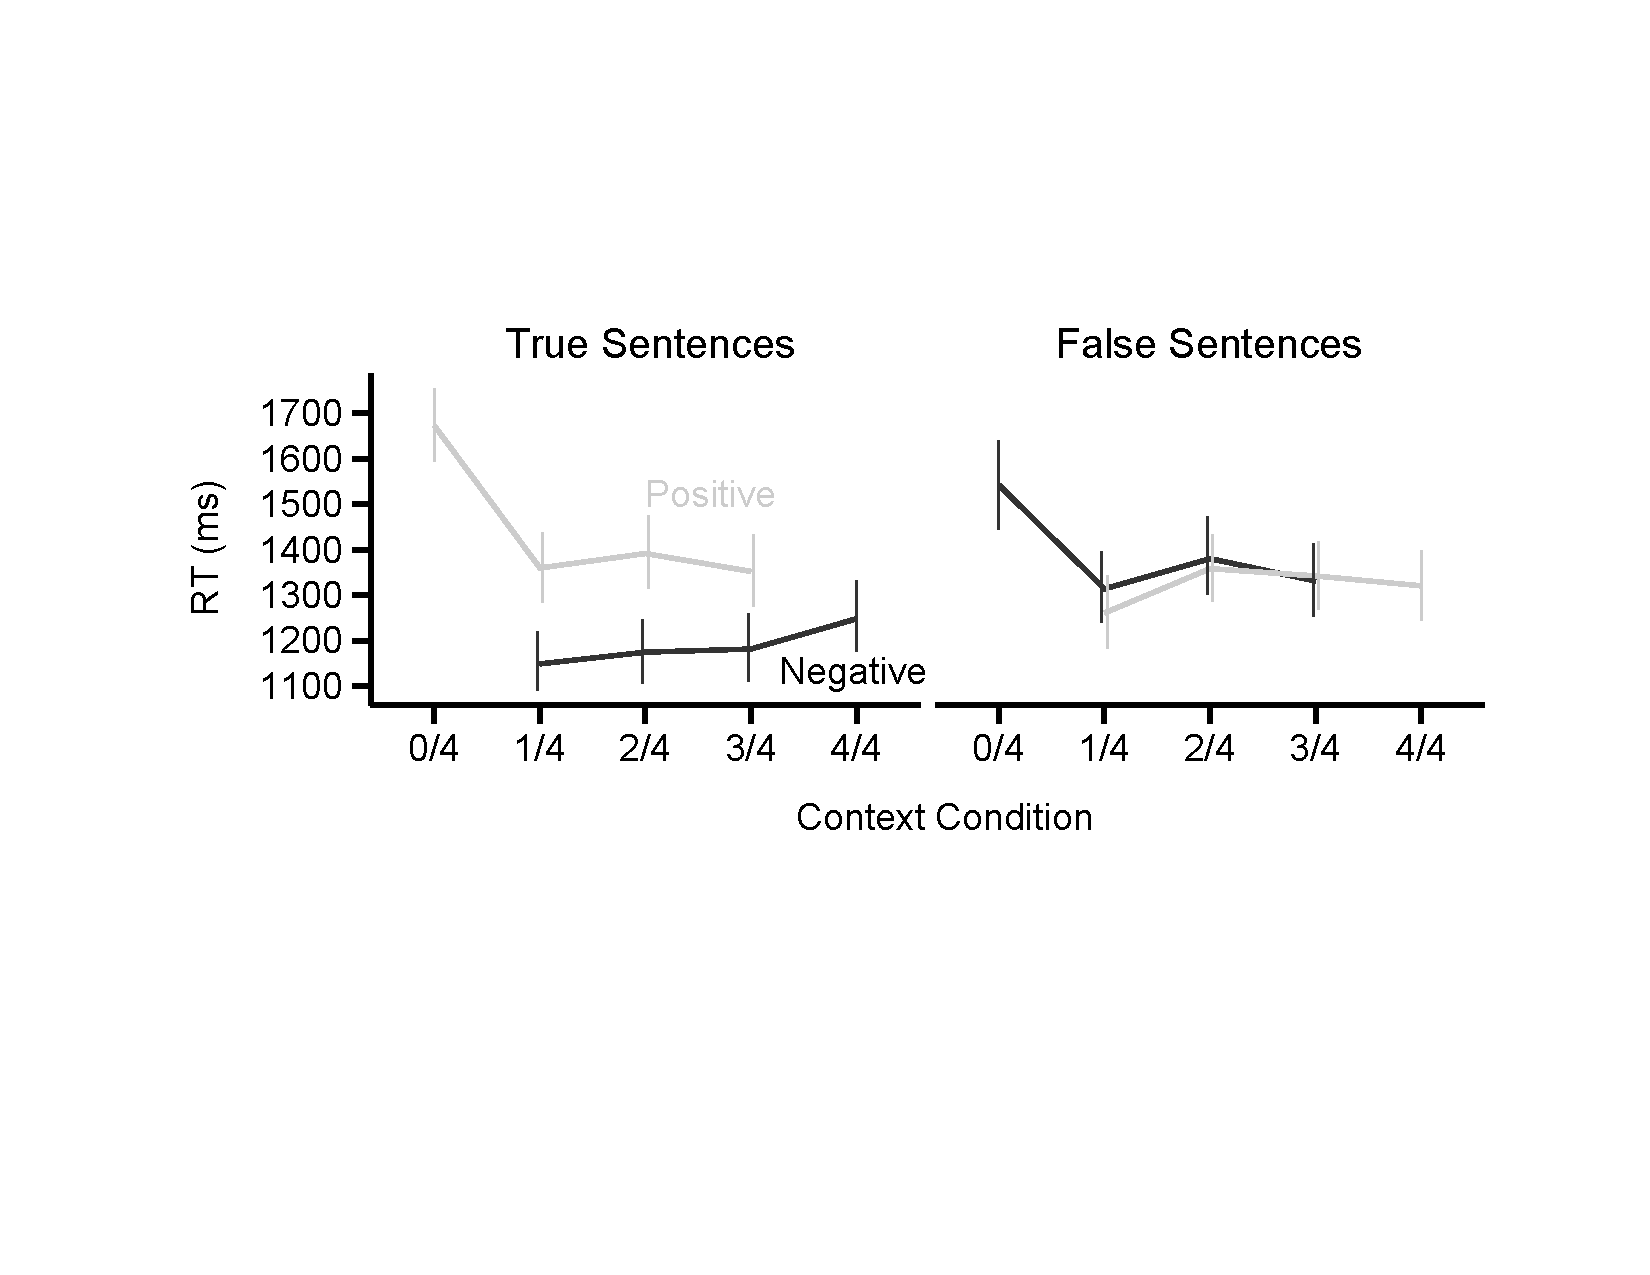
\includegraphics[width=6in]{figures/rts.pdf}
\caption{\label{fig:e2line} Reaction times for each trial type across different conditions. Responses to true sentences are shown on the left, and false sentences are shown on the right.  Negative sentences are shown in grey, and positive sentences in black.  The context condition is notated by a fraction representing the number of characters in the context who held target items. Error bars show 95\% confidence intervals computed by non-parametric bootstrapping.  }
\end{center} 
\end{figure}

Participants were fastest to respond to true positive sentences, and slowest to respond to true negative sentences.  Responses to true negative sentences showed the most pronounced effect of context, with reaction times in response to negative sentences decreasing as the proportion of target items in the context increased.  Responses to false positive sentences showed a similar but less pronounced effect of context, and responses to true positive and false negative sentences showed a slight but reversed effect of context, with increased reaction times as the proportion of target items in the context increased.  

To evaluate the reliability of these patterns, we fit a linear mixed-effects model to reaction times in response to sentences.  We examined the interaction between sentence type (i.e. positive or negative sentences), truth value (i.e. true or false sentences), and context condition on reaction times.\footnote{All mixed-effects models were fit using the lme4 package version 1.1-7 in R version 3.1.2.  The model specification was as follows: \texttt{RT $\sim$ sentence~$\times$~truth~$\times$~context + (sentence~\textbar~subject) +  (sentence~\textbar~item)}.  Significance was calculated using the standard normal approximation to the $t$ distribution \cite{barr2013}. Data and analysis code can be found at FILL THIS IN LATER.}  Results of this model showed an interaction between sentence type and truth value, such that true positive sentences elicited the fastest responses and true negative sentences elicited the slowest responses ($\beta= 895$, $p< .001$).  The model showed a significant negative linear effect of context, with reactions times decreasing as the proportion of characters with target items increased ($\beta= -59$, $p< .001$), but a significant three-way interaction between sentence type, truth value, and context indicates that this is driven primarily by responses to true negative sentences $\beta= -209$, $p< .001$), with true positive and false negative sentences showing a smaller positive linear effect of context.  

\begin{table}[t]
\caption{Coefficient estimates from a mixed-effects model predicting listeners' reaction times in response to sentences in different context conditions.}
\begin{center}
\small\addtolength{\tabcolsep}{-5pt}
\begin{tabular}{rrrr}
  \hline
 & Coefficient & Std. err. & t value \\ 
  \hline
(Intercept) & 1541 & 45 & 34.20 \\ 
  Sentence (Negative) & -282 & 50 & -5.63  \\ 
  Truth value (True) & -461 & 50 & -9.29 \\
  Context & -59 & 11 & -5.44 \\ 
  Sentence$\times$Truth value & 895 & 71 & 12.65 \\
  Sentence$\times$Context & 78 & 15 & 5.05 \\
  Truth value$\times$Context & 92 & 15 & 5.97 \\
  Sentence$\times$Truth value$\times$Context & -209 & 22 & -9.52 \\
   \hline
\end{tabular}
\vspace{-1.5cm}
\end{center}
\end{table}

\subsection{Speaker Condition}

\begin{figure}[t]
\begin{center} 
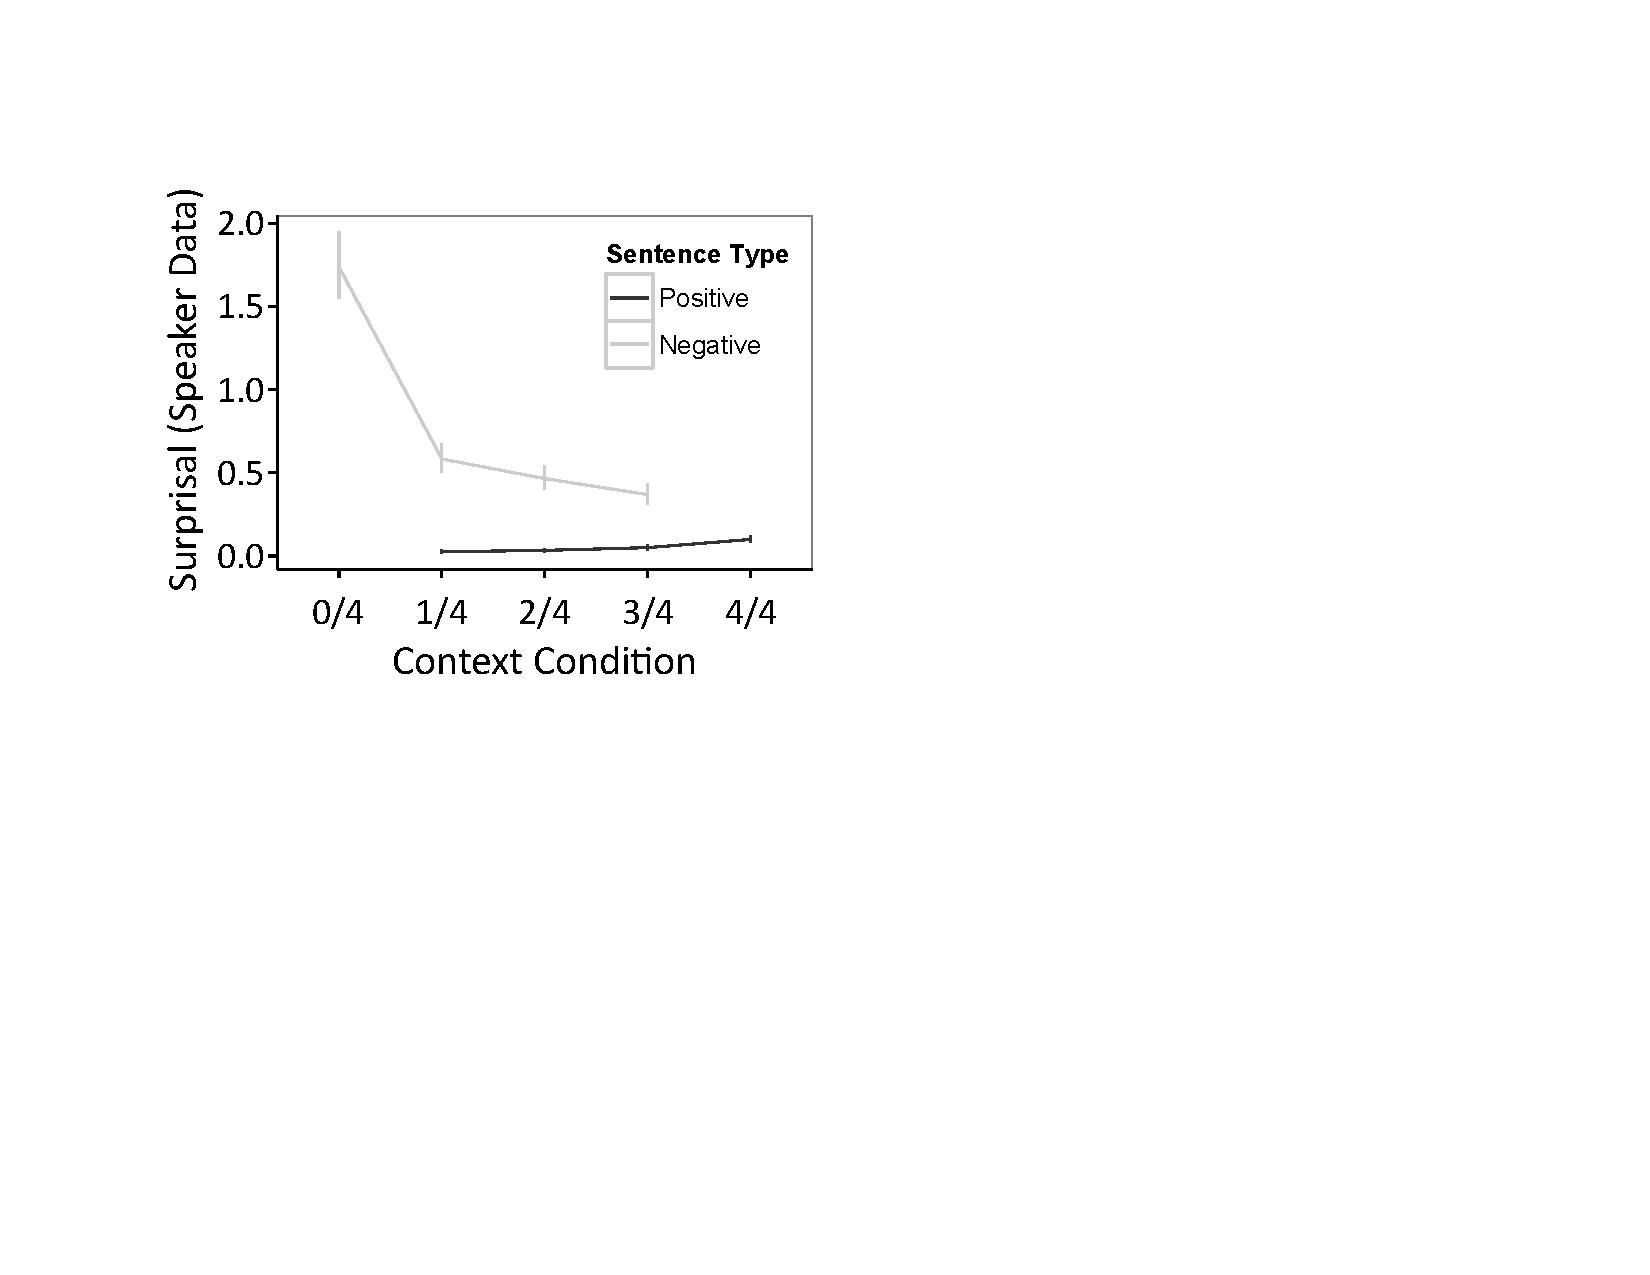
\includegraphics[width=6in]{figures/surprisals.pdf}
\caption{\label{fig:e2line} Surprisal for true positive and true negative sentences across different conditions. On the left is a plot of surprisal computed using data from the speaker condition of the experiment, and on the right are model predictions for the same sentences.  Negative sentences are shown in grey, and positive sentences in black.  The context condition is notated by a fraction representing the number of characters in the context who held target items. Error bars show 95\% confidence intervals computed by non-parametric bootstrapping.  }
\end{center} 
\end{figure}

We hypothesized that the processing cost of negation could be explained by the Gricean intuition that listeners expect speakers to produce informative utterances.  To link pragmatic expectations to reaction time, we assume that reaction time is proportional to \emph{surprisal}. Surprisal is an information-theoretic measure of the amount of information carried by an event (in this case, an utterance in some context) based on its probability. Surprisal has been used effectively to predict reaction times from probabilistic models \cite{levy2008}; here, we used the probability of participants in the speaker condition producing a true positive or a true negative utterance in different contexts to calculate pragmatic surprisal.

Surprisal was much higher for negative sentences compared to positive sentences across all context conditions.  Negative sentences in the $\frac{0}{4}$ condition had the highest surprisal, and positive sentences in the $\frac{1}{4}$ condition had the lowest surprisal.  For negative sentences, surprisal decreased as the number of characters with target items increased, and for positive sentences surprisal increased as the number of characters with target items increased.  

%More here
To test the hypothesis that sentence processing is related to listeners' expectations about what a speaker will say, we plotted the mean reaction time in response to true positive and negative utterances in each condition against the surprisal for the same utterances.  There was a significant posiitve correlation between surprisal and reaction time for true negative sentences, $r=.97$, $p<.001$, supporting our prediction that the effects of context on reaction time were driven by differences in how speakers' described the stimuli.  

%\section{Discussion}



%Quantitative manipulation of the strength of the context resulted in systematic changes in the processing cost of negation, particularly for true negative sentences.  This finding is consistent with our initial hypothesis: As the proportion of people in the context with the target item increases, describing the trial picture as \emph{not} having that target item becomes more informative.  That is, the more people in the context who have apples, the more we expect a person with nothing to be described as ``a boy with no apples.'' 

%FIXME: NEED MORE HERE -- Make a point about this being a general pragmatic process.  

%\section{Experiment 2}
%
%In Experiment 1, we demonstrated that a simple visual context can facilitate the processing of negative sentences, and that there is a linear relationship between the strength of the context and the effect on reaction time to evaluate negative sentences.  Contexts that set up a strong expectation lead to faster reaction times to process a negative sentence when that expectation is violated.  Our prediction was based on previous work demonstrating that participants expect speakers to be informative when speaking \cite{frank2012}.  If everyone in the context has a specific feature, and the trial character is lacking that feature, it is highly informative to describe the trial character in terms of the negation of the expected feature.  However, although the results of Experiment 1 support this interpretation, we do not know for sure whether participants expect speakers to use negation in these contexts.  Experiment 2 attempts to directly measure participants' expectations of how a speaker would describe the pictures seen in Experiment 1.
%
%\subsection{Method}
%
%\subsubsection{Participants} 
%
%%NOTE: These ns are correct & checked
%We recruited 296 participants from mTurk (167 male, 127 female, two declined to report gender; ages 18 -- 65+). We restricted participation to individuals in the US and paid 50 cents for this 10 minute study.  
%
%\subsubsection{Stimuli}
%
%FIXME: ADD STIMULI FIGURE
%
%Stimuli were identical to those used in Experiment 1, with the same within-subjects context condition.  The only difference was that after the target item was highlighted in red, an incomplete sentence appeared (e.g. ``[NAME] has $\rule{3cm}{0.15mm}$.'').  In half of the trials, the highlighted picture was holding target items, and in half of the trials, the highlighted picture was holding nothing.  The experiment was fully crossed such that target characters appeared with or without target items an equal number of times in each context type.  
%
%\subsubsection{Procedure}
%
%Participants were first presented with an instructions screen which described the task and informed them that they could stop at any time.  
%
%In each trial, participants saw an array of four pictures: The target pictures and three context pictures presented in a random order.  Participants were told to look at these pictures for four seconds, at which point a red box appeared around one of the pictures.  One second later, an incomplete sentence appeared.  Participants were told to finish the sentence (by typing into a small text box) using only a few words, in a way that would help someone else identify the character in the red box if they saw the pictures in a different order.  
% 
% \subsubsection{Data Processing}
%We excluded 13 participants who did not list English as their native language, leaving a total of 283 participants for analysis.  
%
%\subsection{Results and Discussion}
%
%
%FIXME: NEW GRAPHS
%\begin{figure}[t]
%\begin{center} 
%\includegraphics[width=3.25in]{figures/study2a_linegraph.pdf}
%\includegraphics[width=3.25in]{figures/study2b_linegraph.pdf}
%\caption{\label{fig:e2line} Reaction times for each trial type across different conditions. Responses to true sentences are shown on the left, and false sentences are shown on the right.  Negative sentences are shown in grey, and positive sentences in black.  Data for Experiment 2a (3-person contexts) are shown above, and data for Experiment 2b (4-person contexts) are shown below.  The context condition is notated by a fraction representing the number of characters in the context who held target items. Error bars show 95\% confidence intervals.  }
%\end{center} 
%\end{figure}
%
%FIXME: WHAT RESULTS HERE?
%
%FIXME:
%In Experiment 1, we found that including a visual context facilitates the processing of negative sentences, and that this effect is modulated by the strength of the expectation set up by the context.  As the proportion of people with a target item in the context increases, the reaction time to process a negative sentence that negates that target property decreases.  We hypothesized that this effect is due to the ways that context changes expectations about what a speaker might say to describe a picture.  If you see a context in which the every character except for one is holding apples, it makes sense to predict that the boy holding nothing might be described as a ``boy with no apples''.  However, if you see a context in which nobody is holding anything, it would be odd to describe one of them as ``a boy with no apples'', because you have no reason to expect that he \emph{would} have apples.  Our prediction was that these expectations, calculated as the surprisal of seeing a picture described using a certain sentence, would be positively correlated with reaction times from previous studies.  Experiment e confirmed this hypothesis.  

%\section{Model}
%NOTE: This might be too weird, but I skipped straight to the model here because otherwise I felt like there was too much repetition of the discussion of experimental results?  


%Our experiment showed that participants were faster to respond to and more likely to produce negative sentences when a greater proportion of characters in the context possessed the negated item.  This was consistent with our hypothesis that the processing cost of negation is due to general pragmatic principles about how listeners expect speakers to behave.  
%that a simple visual context can facilitate the processing of negation, with contexts that set up a strong expectation leading to faster RTs for negative sentences in the listener condition.  In the speaker condition, we used participants' spontaneous descriptions of our stimuli to calculate the surprisal of different sentence types, and demonstrated that participants' reaction times are highly correlated with the surprisal of an utterance. 
%We hypothesized that this effect was driven by the expectation that speakers are informative \cite{grice1975,frank2012}: If everyone in a context has a specific feature except for the person being described, it is highly informative to describe that person in terms of the negation of the expected feature. In contrast, if no one has a feature, it's pragmatically odd to negate it. In this section, we formalize these intuitions.  

%We modeled the behavior of participants in our experiments by assuming that reaction time is proportional to the surprisal of the utterance $w$, given the context $C$ and the speaker's intended referent $r_S$ (following \citeNP{levy2008}):

%\begin{equation}\label{eq:model_surprise}
%RT \sim -\log(P(w| r_s, C)).
%\end{equation}

%\noindent We then define the probability of the utterance as proportional to its utility (following \citeNP{frank2012}):
%
%\begin{equation}\label{eq:pw1}
%P(w | r_s, C) \propto  e^{U(w;r_s,C)},
%\end{equation} 
%
%\noindent This utility is defined as the informativeness of $w$ minus its cost $D(w)$:
%
%\begin{equation}\label{eq:utility}
%U(w;r_s,C) = I(w;r_s, C) - D(w).
%\end{equation}
%
%\noindent Informativeness in context is calculated as the number of bits of information conveyed by the word. We assume that $w$ has a uniform probability distribution over its extension in context (e.g.\ ``boy with apples'' applies to any boy who has apples, leading to a probability of $1/|w|$ of picking out each individual boy with apples) :
%
%\begin{equation}\label{eq:info}
%I(w;r_s, C) = -(-\log(|w|^{-1})).
%\end{equation}
%
%\noindent The cost term $D(w)$ can then be defined in any number of ways; in this model we define it as the number of words in the utterance multiplied by a cost-per-word parameter.  Note that in our experiment, the negative sentences always have exactly one word more than the positive sentences. 
%
%We created a sparse vocabulary which represented possible words to describe the characters.  This included the target utterance (e.g.\ ``apples'' and ``no apples''), as well as words that were uniformly true or false of all characters. Combining Equations \ref{eq:pw1}--\ref{eq:info}, and normalizing Eq.\ \ref{eq:pw1} over all possible words in the vocabulary $V$, we have:
%
%\begin{equation}\label{eq:pw2}
%P(w | r_s, C) = \frac{ e^{\log(|w|^{-1}) - D(w)}} {\sum_{w' \in V}{e^{\log(|w'|^{-1}) - D(w')}}}.
%\end{equation}
%
%\noindent Combining Eq. \ref{eq:model_surprise} with Eq. \ref{eq:pw2}, this model predicts that as the number of e.g.\ boys with apples in the context increases, the informativeness of the negative sentence ``Bob has no apples'' increases, because it selects an increasingly smaller subset of the context. Highly informative sentences will have high probability, hence lower surprisal and faster RTs. 
%
%We fit this model to the data from our experiment, with cost = 2.1.\footnote{We present the results of our simulations using the best-fitting parameters, but the model predictions remain stable over a wide range of parameter values with cost > 1).}  Our model accounted for a substantial amount of variance in reaction times for participants in the listener condition ($r=.89$, $p<.01$) as well as surprisal calculated from participants responses in the speaker condition ($r=.81$, $p<.05$).  These results collectively suggest that  speakers' productions are influenced by the informativeness of a sentence in context, and that listeners expect to hear sentences that are more informative given the context.

\section{General Discussion}

We found that participants were faster to respond to and more likely to produce negative sentences when a greater proportion of characters in the context possessed the negated item.  This was consistent with our hypothesis that the processing cost of negation is due to general pragmatic principles about how listeners expect speakers to behave.  We suggested a Gricean account of these data: The processing cost of negation is related to the degree to which it violates expectations about communication in context. In our studies, by changing the proportion of people in the context who held a target item, we systematically manipulated participants' contextual expectations.  We found a parametric relationship between the strength of the context and reaction times, and this relationship was well fit by participants' descriptions of the stimuli in different contexts.

Previous work on sentence processing has suggested that processing negation is fundamentally difficult, perhaps due to the processing cost of negating a proposition (e.g.\ \citeNP{hclark1972}) or the cost of suppressing an affirmative representation (e.g.\ \citeNP{kaup2003}).  Our work here suggests that the difficulty of negation may not be unique to negation at all; instead, general pragmatic mechanisms could be driving this effect.  Due to the specific pragmatics of negation, negative sentences presented without context are uninformative and are thus unlikely to be produced, leading to increased surprisal and slower processing times.  In conversation, however, negative sentences are often produced when some expectation has been violated, decreasing surprisal and processing time.  

What is the mechanism by which context influences the probability of producing a negative utterance?  One possibility is that negative sentences are more informative in contexts that set up a strong expectation that is violated. If the processing cost of negation is pragmatic, then more informative negative sentences should elicit smaller reaction times.  Recent modeling work quantifies pragmatic reasoning in simple experimental contexts \cite{frank2012,goodman2013}. The assumption underlying this work is that speakers are informative---they will produce utterances that will pick out smaller subsets of the context, leaving as little ambiguity as possible for the listener.  This prediction is reflected in our results: True negative utterances were more informative in contexts where more people possessed the negated item, and these contexts elicited the highest rate of negation from speakers and the fastest reaction times from listeners. Another possibility is that a speaker's utterance are influenced by the ``Question Under Discussion'' (QUD; \citeA{roberts1996}). In our experiment, articipants were slowest to respond to trials where none of the characters possessed the objects that were mentioned in the sentence; e.g. ``Bob has/has no apples'' in response to a context where none of the boys are holding anything.  In addition to being uninformative, these sentences might have incurred additional processing costs due to the mention of an unexpected topic.  

%Our analyses focused on true sentences, because of our interest in exploring participants' expectations about how an informative speaker should behave.  Due to the nature of our task, participants in the listener condition likely expected some of the sentences to be false, but it is not clear what constitutes an ``informative'' false sentence.  Our listener data replicate an interaction between sentence type and truth value that is seen frequently in literature on sentence verification tasks \cite{hclark1972}, with false positive sentences showing a similar pattern as true negative sentences.  


Although our specific focus was to understand the processing of negative sentences, this work has implications for sentence processing more generally.  Debates about the effects of pragmatics on linguistic processing exist in other domains, such as the processing of scalar implicatures, \citeNP{huang2009, huang2011, grodner2010}.  For example, \citeA{tomlinson2013} present mouse-tracking data to argue that that processing scalar implicatures is cognitively demanding. Their data, however, are also consistent with our hypothesis that listeners' responses to different sentences are influenced by pragmatic surprisal; in their experiments, participants showed the same mouse-tracking patterns in response to underinformative scalar implicatures as well as underinformative negative utterances.  We believe that formal models of pragmatics can provide insight into these debates and, more generally, into the role that pragmatic context plays in linguistic processing. 
 


\bibliographystyle{apacite}

\setlength{\bibleftmargin}{.125in}
\setlength{\bibindent}{-\bibleftmargin}

\bibliography{negation}

\end{document}